\section{An abstract machine for switches}
\label{s:absmachine}

\begin{figure*}[!t]
  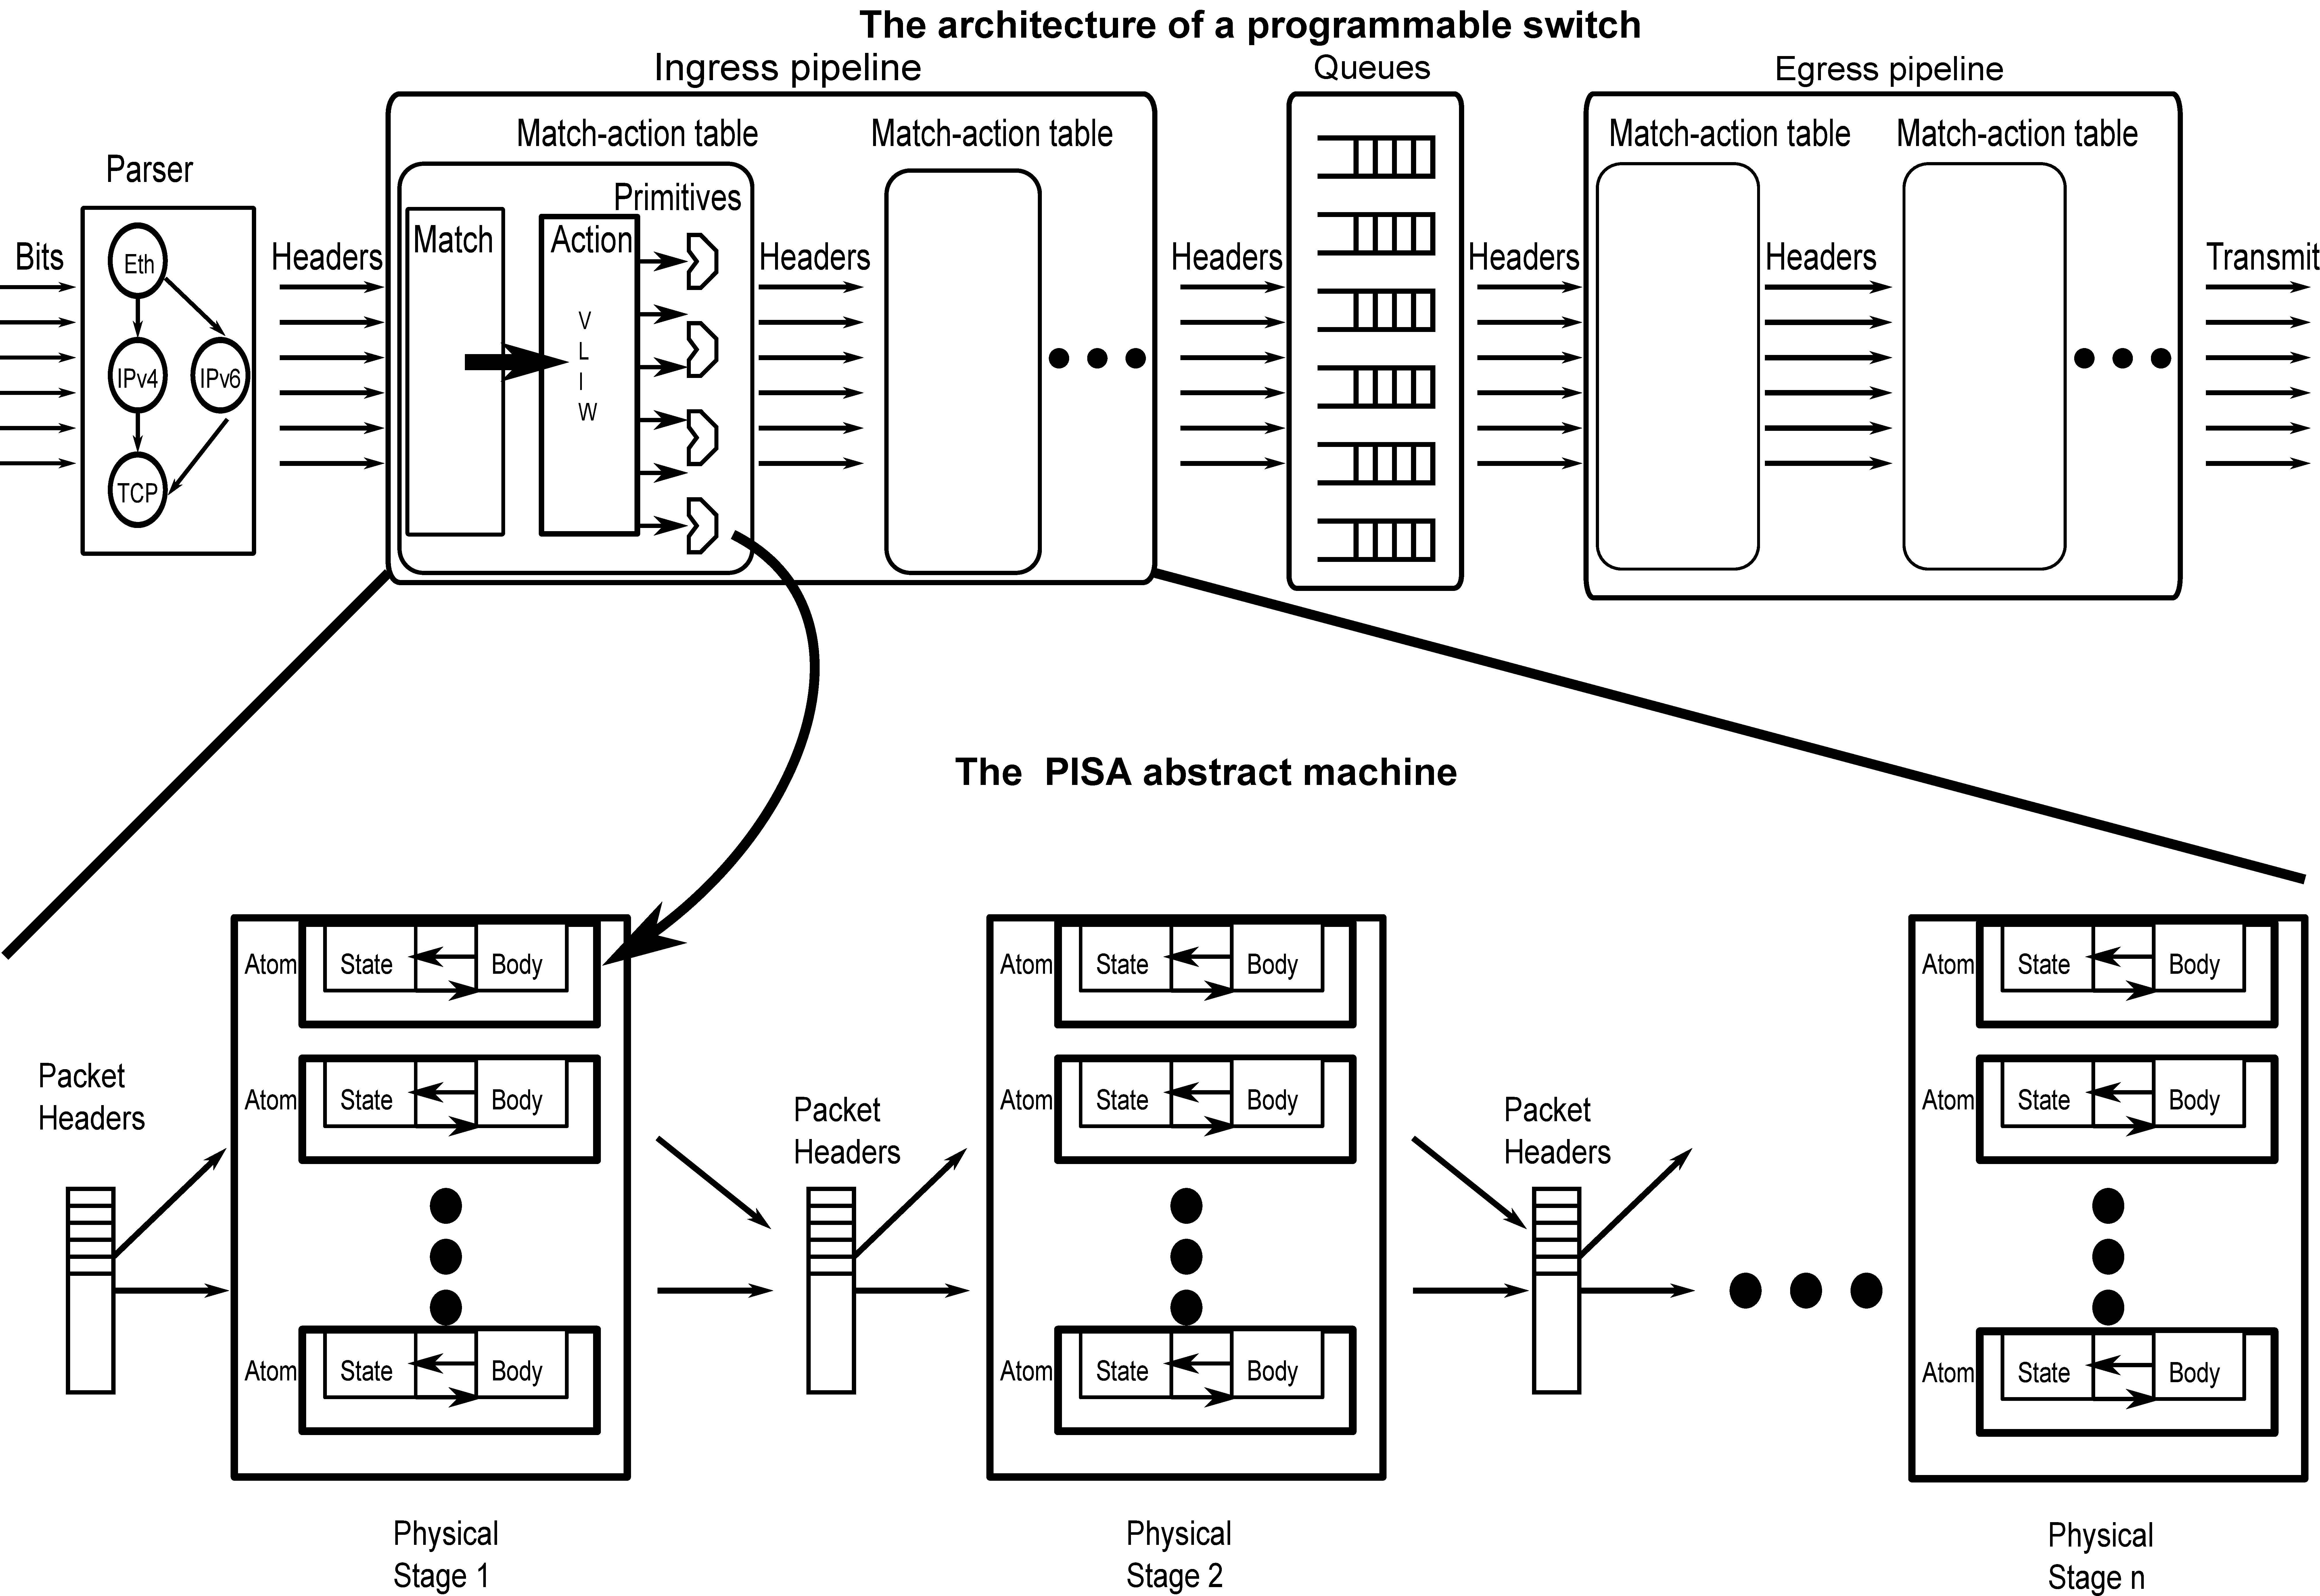
\includegraphics[width=\textwidth]{pisa.pdf}
  \caption{The \absmachine abstract machine and its relationship to
  programmable switch architectures.}
  \label{fig:switch}
\end{figure*}

%TODO: Don't call this an abstract machine. I think that's part of the problem.
% Altenate name: architecture, machine model, and ...?
% People think of this as an IR / portable abstract machine, as opposed to an actual model of the hardware.
% I think that's what triggers the comparisons to NetASM.
%TODO: Mention the differences between stateful and stateless atoms.
This section describes \absmachine (Protocol-Independent Switch Architecture), a
family of abstract machines for programmable switches that differ in the
computational capabilities they provide.  \footnote{The term PISA was briefly
  introduced in a workshop talk~\cite{nick_p4}.  Here, we develop PISA more
completely as a \textit{fully executable} computational model for programmable
switches.} \absmachine machines serve as compiler targets for \pktlanguage
programs.  \absmachine's design abstracts and generalizes line-rate
programmable switch architectures, such as RMT~\cite{rmt}, Intel's
FlexPipe~\cite{flexpipe}, and Cavium's XPliant Packet
Architecture~\cite{xpliant}, which we outline briefly first.

\subsection{Programmable switch architectures}
Programmable switches follow the switch model shown at the top of
Figure~\ref{fig:switch}.  Packets arriving to the switch are parsed by a
programmable parser that turns packets into header fields. These header fields
are first processed by an ingress pipeline consisting of match-action tables
arranged in stages.  Following the ingress pipeline, the packet is queued. Once
the packet is dequeued by the switch scheduler, it is processed by a similar
egress pipeline before being transmitted from the switch.

To reduce chip area, the ingress and egress pipelines are shared across the
switch's ports. This results in demanding requirements on either pipeline.
Each pipeline needs to handle aggregate traffic belonging to all ports on the
switch, regardless of packet size. For instance, for a 64-port switch with each
port running at 10 Gigabits / second and a minimum packet size of 64 bytes
would result in a aggregate packet processing requirement of 1.25 Billion
Packets per second. Equivalently, each pipeline stage needs to process a packet
once every 800 ps.

This budget of 800 ps per packet in each stage greatly curtails the kinds of
operations that can be performed on each packet in a given stage. In contrast
to a software router, NPU, or FPGA, a programmable switch provides a very
limited repertoire of primitives or processing units that can manipulate
packets in each pipeline stage. A switch's primitives determine the set of
algorithms that can be run on it. The technical challenge here is to build a
compiler that can automatically determine the primitives that need to be used
to implement a data-plane algorithm from a high-level description of the
algorithm.

\subsection{The \absmachine abstract machine}

\absmachine (the bottom half of Figure~\ref{fig:switch}) models a switch
pipeline such as the ingress or egress pipeline. A pipeline in \absmachine
consists of a number of pipeline stages that execute synchronously on every
time step. An incoming packet is processed by each stage and handed off to the
next, until it exits the pipeline. Each stage has one time step of latency. For
the example above with 64 ports each running at 10 Gigabits / second, this time
step is 800 ps.

\absmachine only models components pertinent to data-plane algorithms. It
models the computation within a match-action table in a stage (i.e., the action
half of the match-action table), but not the match semantics (e.g., direct,
ternary, or longest prefix). It is easy to embed these actions within a
match-action pipeline by making them default actions~\cite{p4spec} for each
table. \absmachine also does not model packet parsing and assumes that packets
arriving to it are already parsed.

\subsection{Atoms: \absmachine's processing units}

% TODO: Example of why we need this entire language to express atoms.
In \absmachine, each pipeline stage contains a vector of \textit{atoms}. All
atoms in this vector execute in parallel on every time step.  Informally, an
atom is an atomic unit of packet processing that can optionally modify
persistent state stored on the switch, and which the \absmachine machine
supports natively in hardware. Atoms constitute the machine's instruction set.
In contrast to instruction sets for CPUs, GPUs, DSPs, and NPUs, the atoms for a
\absmachine need to be substantially richer. To motivate this, consider a
switch that provides the ability to atomically increment a state variable
stored on the switch to count the number of packets matching a criterion.

Naively, this could be achieved by providing hardware support for three simple
operations: \textit{reading} a piece of memory from one pipeline stage,
\textit{adding} one in the next, and \textit{writing} it back to memory in the
third. However, this doesn't work as we illustrate below.
(Figure~\ref{fig:atomic_increment}).  First, it doesn't provide an atomic
increment: let's say packet 1 increments the counter from 0 to 1 by passing
through the read, add, and write stages in time steps 1, 2, and 3 respectively.
Then, if packet 2 arrives at the read stage at time step 2, it will increment
the counter again from 0 to 1, and write back the value 1 into the write stage.
In effect, this makes it look like there was a single increment when there were
two.

One could imagine providing locks to implement the atomic increment. However,
locking causes contention and in the example above, it would cause packet 2 to
stall, while packet 1's atomic increment completes. This prevents the switch
from processing packets at line rate---something that switches are expected to
attain regardless of the input workload. Finally, practically speaking, share
memory requires building multi-ported memories and routing long wires on the
chip, both of which are hard to do.

% TODO: Continue here.

We represent atoms using a body of sequential code. An atom completes execution
of this body of code and modifies a packet before processing the next packet.
An atom may also contain internal state that persists across packets and
influences the atom's behavior from one packet to the next.  For instance, a
switch counter that wraps around at 100 can be written as the atom
below.\footnote{We use {\tt p.x} to represent field {\tt x} within a packet
{\tt p} and {\tt x} to represent a state variable {\tt x} that persists across
packets.}
  \begin{lstlisting}[style=customc, numbers=none, frame=none]
  if (counter < 99)
    counter++;
  else
    counter = 0;
  \end{lstlisting}
Similarly, a stateless operation that sets a packet field (such as P4's {\tt
modify\_field} primitive~\cite{p4spec}) can be written as the atom below:
\begin{lstlisting}[style=customc, numbers=none, frame=none]
  p.field = value;
\end{lstlisting}

%%\absmachine generalizes several aspects of existing programmable switch
%%architectures. The vector of atoms in each stage generalizes RMT's very-large
%%instruction-word (VLIW)~\cite{rmt} that executes primitive actions on packet
%%fields in parallel. Internal state within an atom models persistent switch
%%state such as meters, counters, and P4's register abstraction~\cite{p4spec} in
%%a unified manner. We assume all state is initialized by the switch control
%%plane, which we don't explicitly model in \absmachine.
%%
\subsection{Computational limits}
\label{s:atomConstraints}

Atoms in \absmachine execute on every time step, reading all packet fields at
the beginning and writing all packet fields at the end of a time step. To
prevent data races, \absmachine forbids two atoms in a stage from writing to
the same packet field.  To provide deterministic performance at line rate,
atoms must be suitably constrained.  We impose two such constraints that
distinguish \absmachine from software routers~\cite{click} and network
processors~\cite{ixp4xx} that sacrifice determinism for programmability.

First, \absmachine machines are \textit{shared-nothing}: each atom maintains a
certain number of state variables that are local to that atom alone. Their
values can be communicated to atoms in subsequent stages only when the values
are copied into packet fields. This restriction reflects the capabilities of
line-rate switches: accessing shared memory from multiple switch stages is
technically challenging because it requires multi-ported RAMs and routing long
wires on the chip.

Second, we constrain the complexity of atoms by defining {\it atom templates}
(\S\ref{ss:code_gen}).  An atom template is a program that always terminates
and specifies how the atom is executed. One example is an ALU with a restricted
set of primitive operations to choose from (Figure~\ref{fig:alu_diag}). Atom
templates allow us to create different \absmachine machines that support
different atoms natively. In practice, we expect such atom templates to be
designed by an ASIC engineer and exposed as part of a \absmachine machine's
instruction set. As programmable switches evolve, the capabilities of atoms
will evolve as well. However, atoms cannot be arbitrarily complex: the line
rate is inversely proportional to an atom's execution
latency~(\S\ref{ss:perfprog}).

\subsection{Resource limits}

